\chapter{Слежение за гармоническим сигналом (регулятор общего вида)}
\label{ch:chap6}

Рассмотрим регулятор общего вида:
$$
H(s) = \frac{\sum^m_{k=0}(b_ks^k)}{\sum^m_{k=0}(a_ks^k)}
$$

Нам нужно определить необходимый порядок $m$, выбрать конкретные параметры $a_k, b_k$, чтобы синтезировать
физически реализуемый регулятор, для следующего задающего сигнала:
$$
g(t) = 2sin(0.5t)
$$
$$
G(s) = \frac{1}{s^2 + 0.25}
$$

Пользуясь принципом внутренней модели из лекции напишем предполагаемый регулятор в общем виде, сразу с учётом того, что он должен быть физически реализуем$(n\geq m)$:
$$
W_{reg}(s) = \frac{k_2s^2 + k_1s + k_0}{s^2 + 0.25}
$$
Как можно заметить, знаменатель мы выбрали таким, что загасить влияние сигнала $g(t)$, который в прошлом задании не давал нам использовать предельную теорему. Мы это увидим далее\dots

$$
\begin{aligned}
  W_{g\to e}(s) = \frac{1}{1 + W} = \frac{1}{1 + \frac{3(k_2s^2 + k_1s + k_0)}{(s^2 + 0.25)(s^2+2.5s+1)}} \\
  W_{g\to e}(s) = \frac{(s^2 + 0.25)(s^2+2.5s+1)}{ (s^2 + 0.25)(s^2+2.5s+1) + 3(k_2s^2 + k_1s + k_0)} 
\end{aligned}
$$
Тогда ошибка слежения будет такова:
$$
E(s) = \frac{(s^2+2.5s+1)}{ (s^2 + 0.25)(s^2+2.5s+1) + 3(k_2s^2 + k_1s + k_0)} 
$$
Тогда предельная теорема:
$$
\lim_{t\to\infty}y(t) = \lim_{s\to 0}sE(s) = \lim_{s\to 0}\frac{(s^3+2.5s^2+s)}{ (s^2 + 0.25)(s^2+2.5s+1) + 3(k_2s^2 + k_1s + k_0)}  = 0
$$
Нам удаётся свести установившуюся ошибку в ноль, но при этом теперь нам нужно подобрать такие коэффициенты регулятора, 
чтобы у нас были только отрицательные полюса, для этого мы раскроем скобки у знаменателя и применим критерий Гурвица:

$$
s^4 + 2.5s^3 + (1.25 + 3k_2)s^2 + (3k_1 + 0.625)s + k_0 + 0.25
$$
Для удобства примем $k_0 = -0.25$, чтобы упростить грядущие равества:
$$
\begin{aligned}
  a_4 = 1, \\
  a_3 = 2.5, \\
  a_2 = 1.25 + 3k_2, \\ 
  a_1 = 3k_1 + 0.625, \\
  a_0 = 0
\end{aligned}
$$
Составим матрицу Гурвица 4-го порядка, а после выпишем с неё угловые миноры\dots
$$
\begin{cases}
  a_1 > 0, \\
  a_1a_2 - a_0a_3 > 0, \\
  a_1a_2a_3 -a_1^2a_4 -a_3^2a_0 > 0
  a_4 > 0
\end{cases}
$$
$$
\begin{cases}
  a_1 > 0, \\
  a_2 > 0, \\
  a_2a_3 -a_1 > 0
\end{cases}
$$
Последнее неравенство решим отдельно:
$$
\begin{aligned}
  \frac{5}{2}(\frac{5}{4} + 3k_2) > 3k_1 + 0.625 \\
  \dots \\
  k_ 1 < \frac{5}{6}(k_2 + 1)
\end{aligned}
$$

\newpage
Проведём несколько опытов:
\begin{figure}[ht]
  \centering
  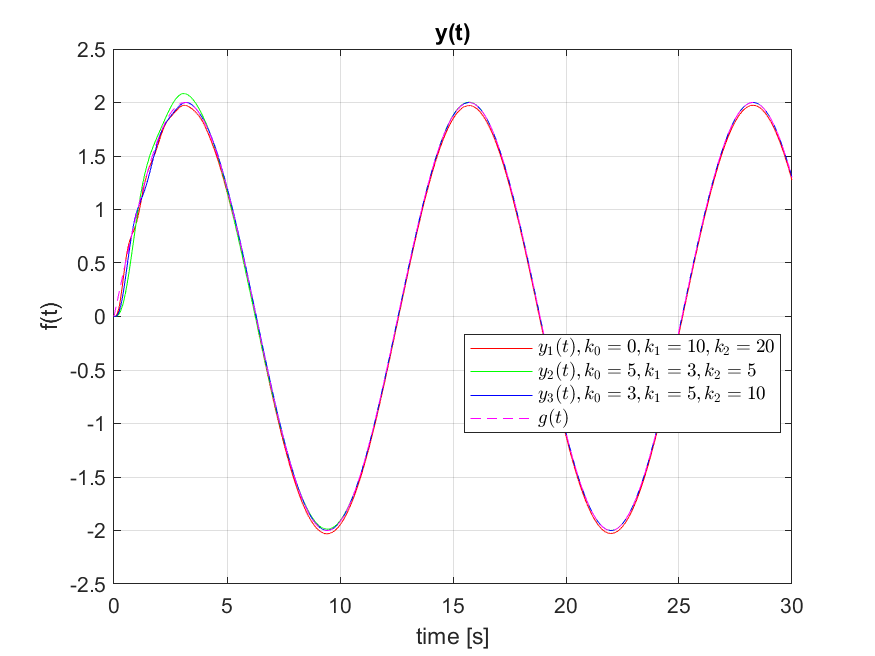
\includegraphics[width=0.8\textwidth]{output_task6_exp1.png}
\caption{Симуляция - гармоническое движение}
\end{figure}

\begin{figure}[ht]
  \centering
  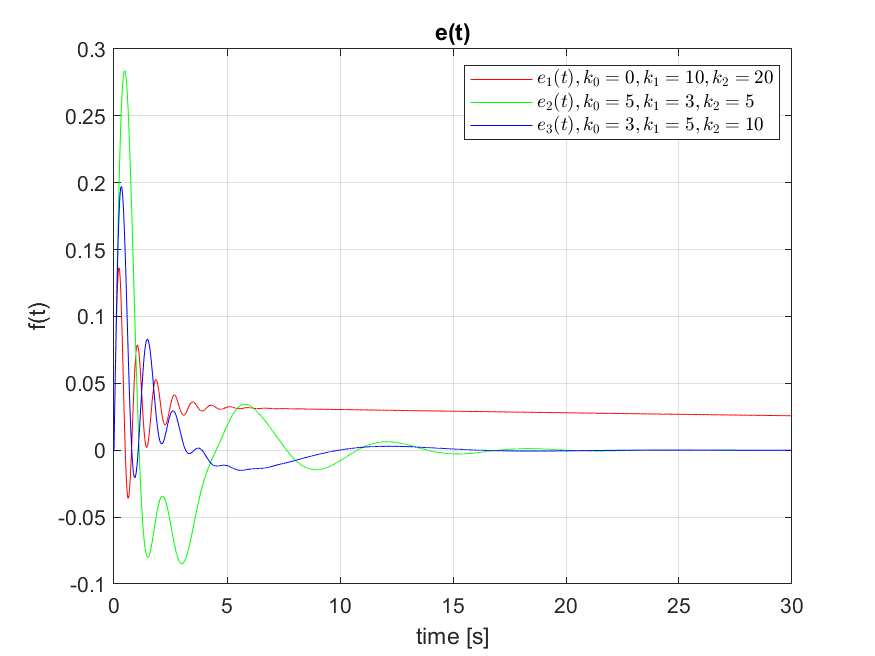
\includegraphics[width=0.8\textwidth]{output_task6_exp2.png}
\caption{Симуляция - гармоническое движение}
\end{figure}
\textbf{Выводы:}  Ошибка системы стремится к нулю, хоть и неохотно(красный график ошибки), на графиках я взял относительно небольшой временной промежуток, чтобы можно было начальные переходные процессы сравнить, далее они все монотонно стремятся к нулю, с разной скоростью. 

Как можно заметить, в моём случае третий параметр $k_0$ довольно сильно доводит переходный процесс до конца, то есть уводит ошибку максимально к нулю.

Мы смогли посчитать установившейся ошибку только из-за того, что построили регулятор таким образом, чтобы сократить мнимый корень из гармонического сигнала знаменателя.

\endinput